\documentclass{article}

% Required packages
\usepackage{amssymb}
\usepackage{amsmath}
\usepackage{graphicx}
\usepackage{geometry}
\usepackage{tikz}
\usepackage{array}
\usepackage{booktabs}
\usepackage{enumitem}
\usepackage{listings}
\usepackage{xcolor}
\usepackage{fancyhdr}
\usepackage{float}
\usepackage{subcaption}
\usepackage{comment}
\usepackage{algorithm}
\usepackage{algpseudocode}
\usepackage{booktabs}
\usepackage{caption}
\usepackage{subcaption}
\usepackage{booktabs}
\usepackage{array}
\usepackage{caption}
\usepackage{graphicx}
\usepackage{siunitx}
\usepackage{graphicx}
\usepackage{siunitx}
\usepackage{array}


% Set page geometry
\geometry{a4paper, margin=1in}

% Configure listings for Python
\lstset{
  language=Python,
  basicstyle=\ttfamily\footnotesize,
  numbers=left,
  numberstyle=\tiny\color{gray},
  frame=single,
  breaklines=true,
  breakatwhitespace=true,
  captionpos=b,
  tabsize=4,
  showspaces=false,
  showstringspaces=false,
  showtabs=false,
  commentstyle=\color{gray}\textit,
  keywordstyle=\color{blue}\bfseries,
  stringstyle=\color{red}
}

\begin{document}

\pagestyle{fancy}
\chead{DSC 257: Unsupervised Learning (Fall 2025)}
\lhead{Homework 5}
\rhead{Randall Rogers}

%------------------
% Solution for 1(a)
%------------------
\subsection*{Solution 1}
\noindent\rule{\textwidth}{0.4pt}\\
\subsubsection*{Solution 1 (a)}
The Gaussian (Normal) distribution $N(\mu, \sigma^2)$ is symmetric about its mean $\mu$. \\
Given $X \sim N(10, 16)$, it follows that the mean is $\mu = 10$.

\begin{align*}
    P(X \geq \mu) = 0.5
\end{align*}
Hence, the probability of the random variable $X$ being greater than or equal to the mean is exactly $0.5$, since the Gaussian distribution is symetric about its mean.

\subsubsection*{\normalfont}{$\therefore$ $P(X \geq 10)$ is $0.5$} \\

\noindent\rule{\textwidth}{0.4pt}\\

\newpage

%------------------
% Solution for 1(b)
%------------------
\subsection*{Solution 1}
\noindent\rule{\textwidth}{0.4pt}\\
\subsubsection*{Solution 1 (b)}
The Gaussian distribution is a continuous probability distribution. For any continuous random variable, the probability of it taking a single, exact value is zero.

\subsubsection*{\normalfont}{$\therefore$ $P(X = 10)$ is $0$}

\noindent\rule{\textwidth}{0.4pt}\\

\newpage

%------------------
% Solution for 1(c)
%------------------
\subsection*{Solution 1}
\noindent\rule{\textwidth}{0.4pt}\\
\subsubsection*{Solution 1 (c)}
We can solve this using the Empirical Rule (68-95-99.7 rule).
Given $X \sim N(10, 16)$, we have $\mu = 10$ and $\sigma = \sqrt{16} = 4$.
We want to find $P(X \geq 14)$, which is $P(X \geq \mu + \sigma)$.


\begin{flushleft}
    The Empirical Rule states that approximately 68\% of the data lies within one standard deviation of the mean.
\end{flushleft}
\begin{align*}
    P(\mu - \sigma \leq X \leq \mu + \sigma) &\approx 0.68 \\
    P(6 \leq X \leq 14) &\approx 0.68
\end{align*}
The total probability outside this range is $1 - 0.68 = 0.32$.
\begin{align*}
    P(X < 6) + P(X > 14) \approx 0.32
\end{align*}
By the symmetry of the Gaussian distribution, the two tail probabilities are equal.
\begin{align*}
    P(X \geq 14) = P(X > 14) \approx \frac{0.32}{2} = 0.16
\end{align*}

\subsubsection*{\normalfont}{$\therefore$ $P(X \geq 14) \approx 0.16$}

\noindent\rule{\textwidth}{0.4pt}\\

\newpage

%------------------
% Solution for 1(d)
%------------------
\subsection*{Solution 1}
\noindent\rule{\textwidth}{0.4pt}\\
\subsubsection*{Solution 1 (d)}
We use the Empirical Rule. Given $X \sim N(10, 16)$, we have $\mu = 10$ and $\sigma = 4$.
We want to find $P(X \leq 2)$, which is $P(X \leq 10 - 8)$ or $P(X \leq \mu - 2\sigma)$.


\begin{flushleft}
    The Empirical Rule states that approximately 95\% of the data lies within two standard deviations of the mean.
\end{flushleft}
\begin{align*}
    P(\mu - 2\sigma \leq X \leq \mu + 2\sigma) &\approx 0.95 \\
    P(2 \leq X \leq 18) &\approx 0.95
\end{align*}
The total probability outside this range is $1 - 0.95 = 0.05$.
\begin{align*}
    P(X < 2) + P(X > 18) \approx 0.05
\end{align*}
By symmetry, the two tail probabilities are equal. We are interested in the left tail.
\begin{align*}
    P(X \leq 2) = P(X < 2) \approx \frac{0.05}{2} = 0.025
\end{align*}

\subsubsection*{\normalfont}{$\therefore$ $P(X \leq 2) \approx 0.025$}

\noindent\rule{\textwidth}{0.4pt}\\

\newpage

%------------------
% Solution for 2(a)
%------------------
\subsubsection*{Solution 2}
\noindent\rule{\textwidth}{0.4pt}\\
\subsubsection*{Solution 2 (a)}
\begin{align*}
    \lambda &= \frac{\sum_{k=0}^{n\geq 9} k \cdot N_k}{\sum_{k=0}^{n\geq 9} N_k} \\
    &= \frac{22 \cdot 0 + 66 \cdot 1 + 106 \cdot 2 + 115 \cdot 3 + 85 \cdot 4 + 55 \cdot 5 + 28 \cdot 6 + 13 \cdot 7 + 10 \cdot 8 + 9 \cdot 0 + \dots}{500} \\
    &= \frac{0 + 66 + 212 + 345 + 340 + 275 + 168 + 91 + 80 + 0}{500} \\
    &= \frac{1577}{500} \\
    &= 3.154
\end{align*}

\subsubsection*{\normalfont}{$\therefore$ the value of $\lambda$ you choose is $3.154$}\\

\noindent\rule{\textwidth}{0.4pt}\\

\newpage

%------------------
% Solution for 2(b)
%------------------
\subsubsection*{Solution 2}
\noindent\rule{\textwidth}{0.4pt}\\
\subsubsection*{Solution 2 (b)}
Let $\lambda = 3.154$ as found in \textit{part (a)}.

\subsubsection*{Poisson pmf Code}
\begin{lstlisting}
import numpy as np
import matplotlib.pyplot as plt
from scipy.stats import poisson

# Parameter from part (a)
lambda_val = 3.154

# k values from 0 to 10
k_values = np.arange(0, 11)

# Calculate Poisson PMF probabilities for each k
probabilities = poisson.pmf(k_values, lambda_val)

# Create the bar plot
plt.figure(figsize=(10, 6))
plt.bar(k_values, probabilities, color='skyblue', edgecolor='black')

# Add labels and title
plt.xlabel('k (Number of Calls in one hour)', fontsize=12)
plt.ylabel('Probability P(X=k)', fontsize=12)
plt.title(f'Poisson PMF for $\lambda = {lambda_val}$', fontsize=14)
plt.xticks(k_values) # Ensure integer ticks on x-axis
plt.grid(axis='y', linestyle='--', alpha=0.7)

# Save the figure
plt.savefig('poisson_pmf.png', dpi=150, bbox_inches='tight')

print("Poisson PMF plot saved as 'poisson_pmf.png'")
# Print probabilities for reference
for k, prob in zip(k_values, probabilities):
    print(f"P(X={k}) = {prob:.5f}")

"""
# output from for loop
P(X=0) = 0.04268
P(X=1) = 0.13462
P(X=2) = 0.21229
P(X=3) = 0.22319
P(X=4) = 0.17598
P(X=5) = 0.11101
P(X=6) = 0.05835
P(X=7) = 0.02629
P(X=8) = 0.01037
P(X=9) = 0.00363
P(X=10) = 0.00115
"""
\end{lstlisting}

\newpage
%------------------
% Solution for 2(b)
%------------------
\subsubsection*{Solution 2}
\noindent\rule{\textwidth}{0.4pt}\\
\subsubsection*{Solution 2 (b)}

\begin{figure}[h]
  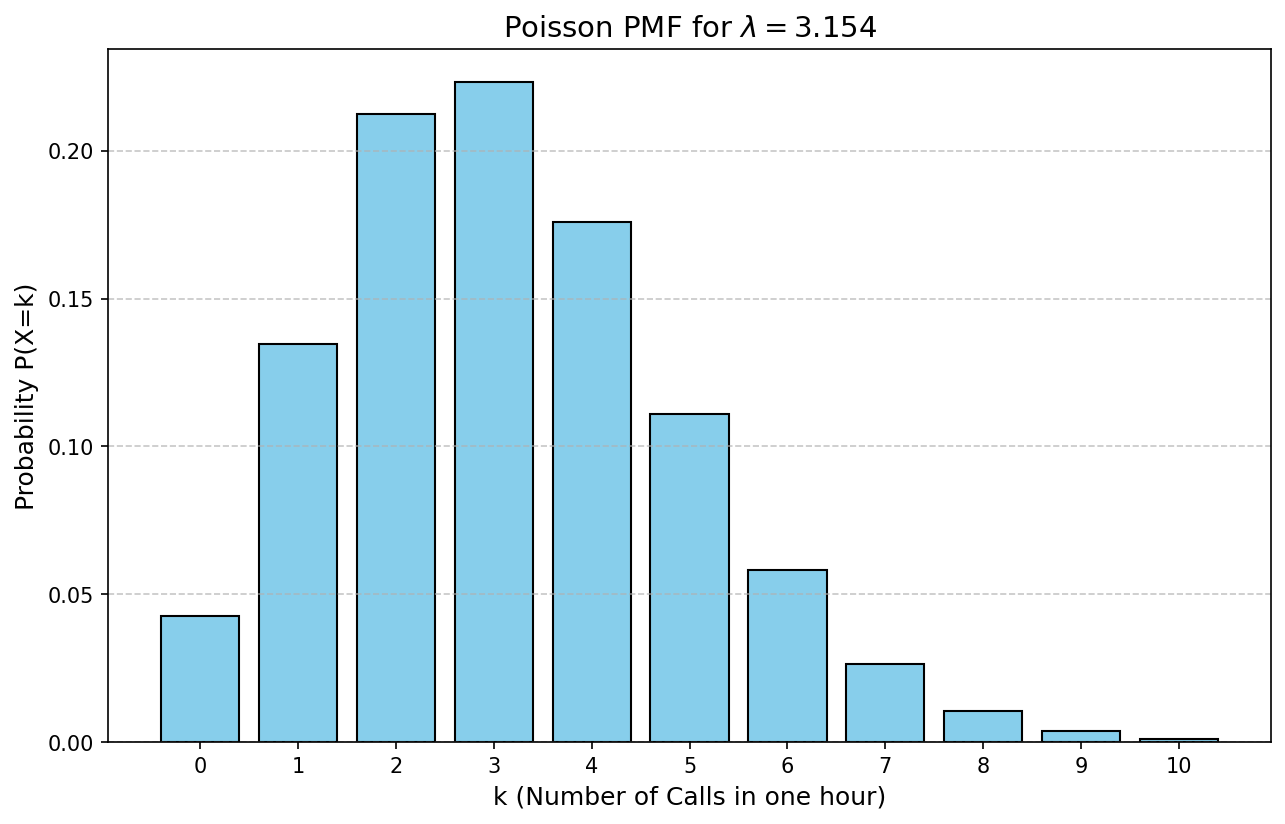
\includegraphics[width=\textwidth]{poisson_pmf.png}
  \caption{Poisson PMF distribution for $\lambda = 3.154$, showing $P(X=k)$ for $k=0...10$.}
  \label{fig:poisson_pmf}
\end{figure}
\noindent\rule{\textwidth}{0.4pt}\\

\newpage

%------------------
% Solution for 2(c)
%------------------
\subsubsection*{Solution 2}
\noindent\rule{\textwidth}{0.4pt}\\

\subsubsection*{Solution 2 (c)}
\begin{flushleft}
    Use the probabilities $P(X=k)$ from \textit{part (b)}and multiply by 500 to find the expected number of one hour intervals during which $k$ calls are recived
\end{flushleft}

\begin{align*}
    P(X=0) &= 0.04268 &\implies E[N_0] = 500 \times 0.04268 &= 21.34 \\
    P(X=1) &= 0.13460 &\implies E[N_1] = 500 \times 0.13460 &= 67.30 \\
    P(X=2) &= 0.21230 &\implies E[N_2] = 500 \times 0.21230 &= 106.15 \\
    P(X=3) &= 0.22310 &\implies E[N_3] = 500 \times 0.22310 &= 111.55 \\
    P(X=4) &= 0.17590 &\implies E[N_4] = 500 \times 0.17590 &= 87.95 \\
    P(X=5) &= 0.11094 &\implies E[N_5] = 500 \times 0.11094 &= 55.47 \\
    P(X=6) &= 0.05830 &\implies E[N_6] = 500 \times 0.05830 &= 29.15 \\
    P(X=7) &= 0.02628 &\implies E[N_7] = 500 \times 0.02628 &= 13.14 \\
    P(X=8) &= 0.01036 &\implies E[N_8] = 500 \times 0.01036 &= 5.18 \\
    P(X \geq 9) &= 1 - P(X \leq 8) = 1 - 0.99448 = 0.00552 &\implies E[N_{\geq 9}] = 500 \times 0.00552 &= 2.76
\end{align*}

\subsubsection*{\normalfont}{$\therefore$ the expected entries are for $\lambda = 3.154$:}
\begin{table}[h]
\centering
\caption{Poisson Distribution and Expected Counts}
\label{tab:poisson_distribution}
\begin{tabular}{c c S[table-format=4.5] S[table-format=3.2]}
\toprule
{$k$} & {$P(X=k)$} & {$E[N_k]$} \\
\midrule
0 & 0.04268 & 21.34 \\
1 & 0.13460 & 67.30 \\
2 & 0.21230 & 106.15 \\
3 & 0.22310 & 111.55 \\
4 & 0.17590 & 87.95 \\
5 & 0.11094 & 55.47 \\
6 & 0.05830 & 29.15 \\
7 & 0.02628 & 13.14 \\
8 & 0.01036 & 5.18 \\
$\geq 9$ & 0.00552 & 2.76 \\
\bottomrule
\end{tabular}
\end{table}

\noindent\rule{\textwidth}{0.4pt}\\

\newpage


%------------------
% Solution for 3(a)
%------------------
\subsubsection*{Solution 3}
\noindent\rule{\textwidth}{0.4pt}\\
\subsubsection*{Solution 3 (a)}
\begin{flushleft}
    For any probability density function (PDF), the total area under the curve must integrate to 1.
\end{flushleft}

$$\int_{-\infty}^{\infty} f(x) \,dx = 1$$

\begin{flushleft}
    We are given the bounds of the probability density function $[0, \lambda]$, so the equation becomes:
\end{flushleft}

\begin{align*}
    \int_{0}^{\lambda} c \,dx &= 1 \\
    c \cdot [x]_{0}^{\lambda} &= 1 \\
    c \cdot (\lambda - 0) &= 1 \\
    c \cdot \lambda &= 1 \\
    c &= \frac{1}{\lambda}
\end{align*}

\subsubsection*{\normalfont}{$\therefore$ the density of $U_{\lambda}$ is $\frac{1}{\lambda}$ and we can express it as $f(x \mid \lambda)$:}

$$
f(x \mid \lambda) = 
\begin{cases} 
      \frac{1}{\lambda} & \text{if } 0 \leq x \leq \lambda \\
      0 & \text{otherwise} 
\end{cases}
$$

\noindent\rule{\textwidth}{0.4pt}\\

\newpage

%------------------
% Solution for 3(b)
%------------------
\subsubsection*{Solution 3}
\noindent\rule{\textwidth}{0.4pt}\\
\subsubsection*{Solution 3 (b)}

We are looking for the value of $\lambda$ that maximizes the likelihood of observing our data $x_{1}, \ldots, x_{n}$.
The likelihood function $L(\lambda)$ is the product of the densities for each observation:
\begin{align*}
    L(\lambda \mid x_1, \ldots, x_n) = \prod_{i=1}^{n} f(x_i \mid \lambda)
\end{align*}
From part (a), we know that the density $f(x_i \mid \lambda)$ is $0$ if any $x_i > \lambda$.
This means that if we choose a $\lambda$ that is *smaller* than even one of our observations, the likelihood $L(\lambda)$ will be 0. This is the minimum possible likelihood, not the maximum.
\begin{flushleft}
    Hence, to have a non-zero likelihood, $\lambda$ must be greater than or equal to *all* observations.
\end{flushleft}

\begin{align*}
    \lambda \geq x_i \quad \text{for all } i=1, \ldots, n
\end{align*}
This is equivalent to saying $\lambda$ must be greater than or equal to the maximum observation:
\begin{align*}
    \lambda \geq \max(x_1, \ldots, x_n)
\end{align*}

\subsubsection*{\normalfont}{$\therefore$ the max likelihood choice of ${\lambda}$ is: }

$$\max(x_1, x_2, \ldots, x_n)$$

\noindent\rule{\textwidth}{0.4pt}\\

\newpage

%------------------
% Solution for 4(a)
%------------------
\subsubsection*{Solution 4}
\noindent\rule{\textwidth}{0.4pt}\\
\subsubsection*{Solution 4 (a)}
We set $k=10$ degrees of freedom. To plot the PDF, we generate a range of $x$ values and use \texttt{scipy.stats.chi2.pdf(x, df=k)} to find the corresponding probability density for each $x$.

\subsubsection*{Chi Squared Code}
\begin{lstlisting}
import numpy as np
import matplotlib.pyplot as plt
from scipy.stats import chi2

# Set degrees of freedom
k = 10

# Create a range of x values
# A chi-squared(k) has mean k and variance 2k.
# So mean=10, std=sqrt(20) approx 4.5.
# We plot from 0 to mean + 4 std (0 to 10 + 18 = 28)
x = np.linspace(0, 30, 400)

# Calculate the PDF values
y_pdf = chi2.pdf(x, df=k)

# Create the plot
plt.figure(figsize=(10, 6))
plt.plot(x, y_pdf, 'r-', lw=2, label=f'Chi-squared PDF (k={k})')

# Add labels, title, and grid
plt.xlabel('X', fontsize=12)
plt.ylabel('Probability Density', fontsize=12)
plt.title(f'Chi-squared Distribution PDF (k={k} degrees of freedom)', fontsize=14)
plt.legend()
plt.grid(True, linestyle='--', alpha=0.7)

# Save the figure
plt.savefig('chi_squared_pdf.png', dpi=150, bbox_inches='tight')

print(f"Chi-squared PDF plot with k={k} saved as 'chi_squared_pdf.png'")
\end{lstlisting}

\newpage

\subsubsection*{Solution 4}
\noindent\rule{\textwidth}{0.4pt}\\
\subsubsection*{Solution 4 (a)}

\subsubsection*{Plot}

\begin{figure}[h]
  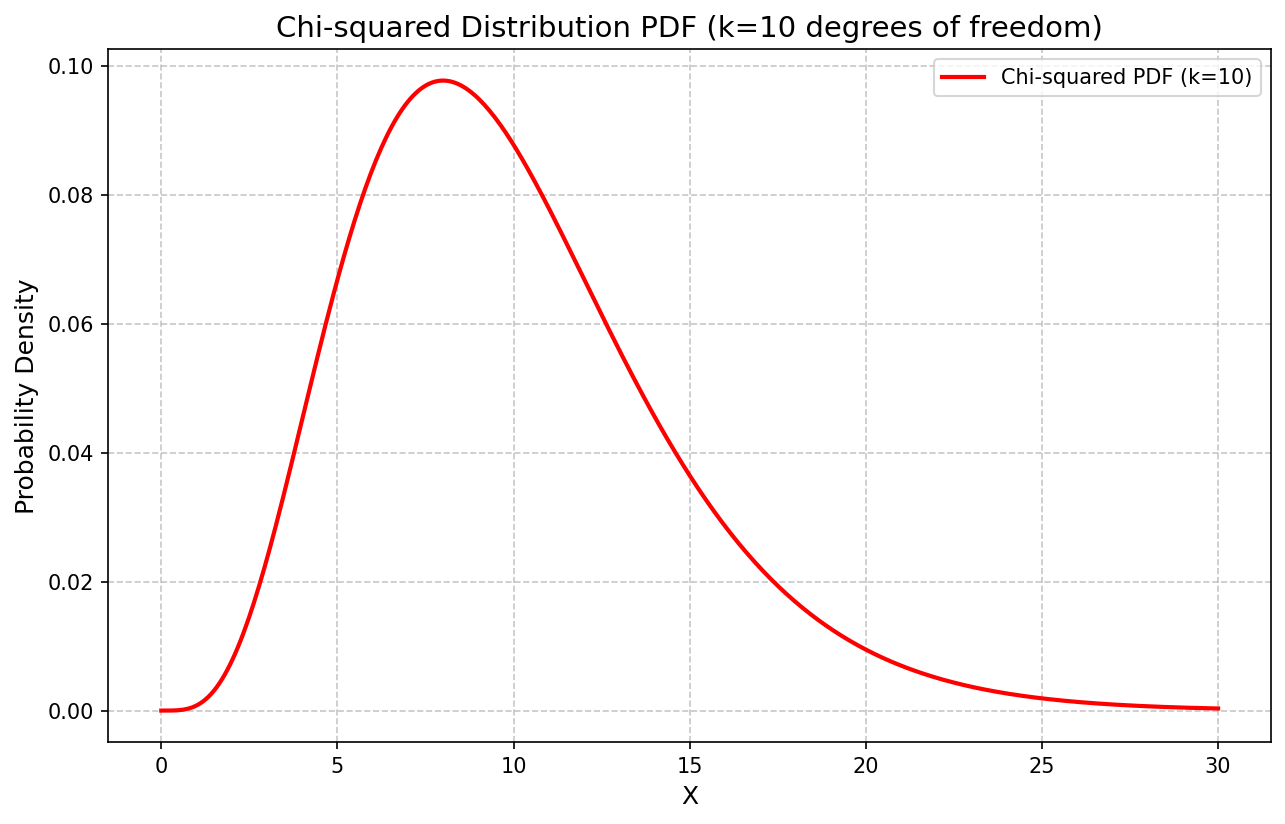
\includegraphics[width=\textwidth]{chi_squared_pdf.png}
  \caption{Chi-squared probability density function (PDF) with $k=10$ degrees of freedom.}
  \label{fig:chi_squared_pdf}
\end{figure}

\noindent\rule{\textwidth}{0.4pt}\\

\newpage

%------------------
% Solution for 4(b)
%------------------
\subsubsection*{Solution 4}
\noindent\rule{\textwidth}{0.4pt}\\
\subsubsection*{Solution 4 (b)}
We use the \texttt{numpy.random.chisquare} function to generate 10,000 samples with $k=10$ degrees of freedom. The median of this sample set is our estimate for the true median of the distribution. We set a random seed for reproducibility. The median is the 50th percentile of the data.
\subsubsection*{Chi Squared Median Code}
\begin{lstlisting}
import numpy as np
import matplotlib.pyplot as plt

# Set parameters
k = 10
num_samples = 10000
random_seed = 42 # For reproducibility

# Set the random seed
np.random.seed(random_seed)

# Generate 10,000 samples from chi-squared(10)
samples = np.random.chisquare(df=k, size=num_samples)

# Estimate the median by finding the median of the samples
median_estimate = np.median(samples)

print(f"Degrees of freedom (k): {k}")
print(f"Number of samples: {num_samples}")
print(f"Estimated Median: {median_estimate:.4f}")

# --- Plotting the histogram and median ---

plt.figure(figsize=(10, 6))
# Plot histogram of the samples
plt.hist(samples, bins=50, density=True, alpha=0.7, 
         label=f'Histogram of {num_samples} samples')

# Plot a vertical line at the estimated median
plt.axvline(median_estimate, color='red', linestyle='--', linewidth=2, 
            label=f'Estimated Median: {median_estimate:.4f}')

plt.xlabel('X', fontsize=12)
plt.ylabel('Density', fontsize=12)
plt.title(f'Median Estimation from $\chi^2(k={k})$ Samples', fontsize=14)
plt.legend()
plt.grid(True, linestyle='--', alpha=0.6)

# Save the figure
plt.savefig('estimate_median.png', dpi=150, bbox_inches='tight')
print("Histogram with median estimate saved as 'estimate_median.png'")
\end{lstlisting}

\newpage

\subsubsection*{Solution 4}
\noindent\rule{\textwidth}{0.4pt}\\
\subsubsection*{Solution 4 (b)}
\subsubsection*{Plot}
\begin{figure}[h]
  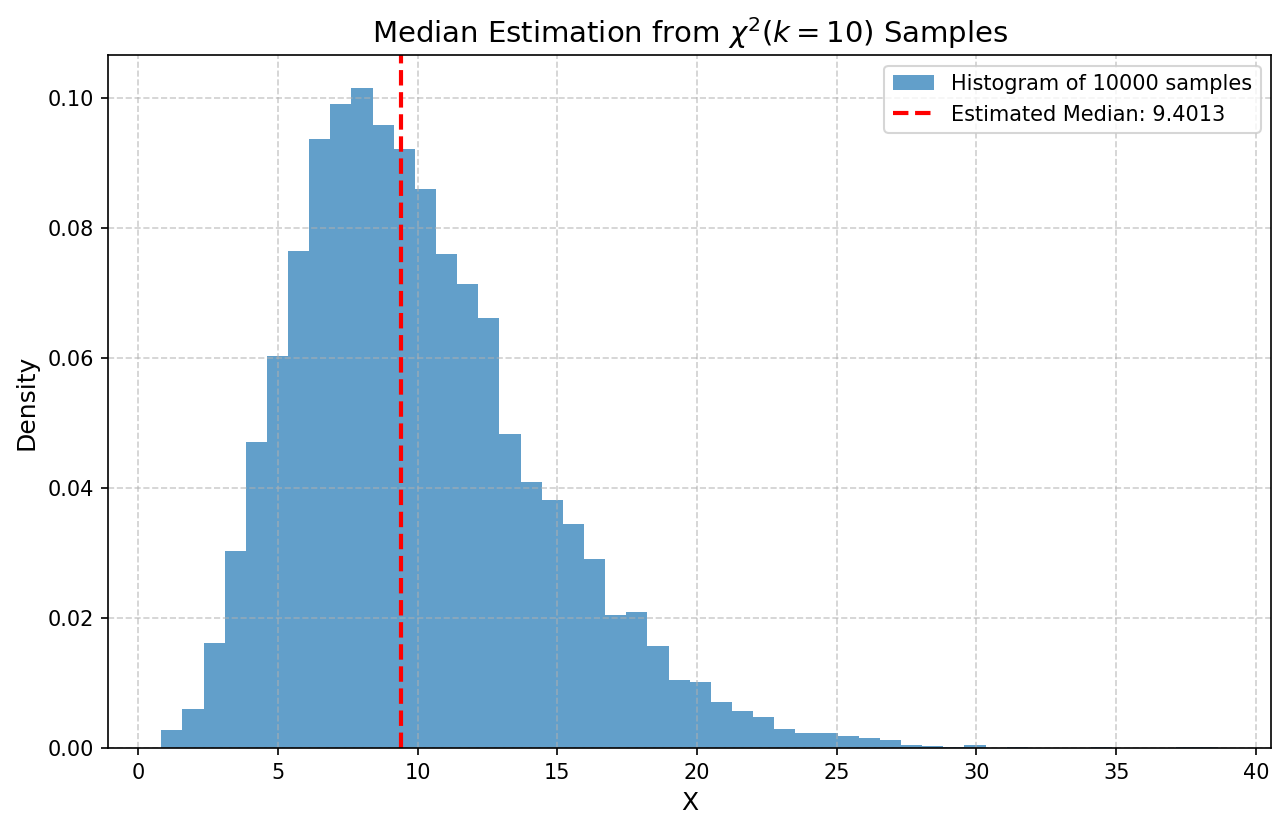
\includegraphics[width=\textwidth]{estimate_median.png}
  \caption{Histogram of 10,000 samples from a $\chi^2(10)$ distribution. The red dashed line shows the estimated median of the samples.}
  \label{fig:estimate_median}
\end{figure}

\subsubsection*{\normalfont}{$\therefore$ The estimated median from 10,000 samples (with seed 42) is $9.4013$.} \\

\noindent\rule{\textwidth}{0.4pt}\\

\newpage

%------------------
% Solution for 5(a)
%------------------
\subsubsection*{Solution 5}
\noindent\rule{\textwidth}{0.4pt}\\
\subsubsection*{Question 5 (a)}
\begin{flushleft}
    \textbf{Maximum likelihood and smoothing.} Upon tossing a coin 20 times, you get heads every time.\\
    How would you estimate the bias (that is, the heads probability) of the coin, using maximum likelihood?
\end{flushleft}

\subsubsection*{Solution 5 (a)}


\subsubsection*{\normalfont}{$\therefore$ the bias of the coin using maximum likelihood is:} \\

\noindent\rule{\textwidth}{0.4pt}\\

\newpage

%------------------
% Solution for 5(b)
%------------------
\subsubsection*{Solution 5}
\noindent\rule{\textwidth}{0.4pt}\\
\subsubsection*{Question 5 (b)}
\begin{flushleft}
    \textbf{Maximum likelihood and smoothing.} Upon tossing a coin 20 times, you get heads every time.\\
    How would you estimate the bias of the coin, using maximum likelihood with Laplace smoothing?
\end{flushleft}

\subsubsection*{Solution 5 (b)}


\subsubsection*{\normalfont}{$\therefore$ the bias of the coin using maximum likelihood with Laplace smoothing is:} \\

\noindent\rule{\textwidth}{0.4pt}\\

\newpage

%------------------
% Solution for 5(c)
%------------------
\subsubsection*{Solution 5}
\noindent\rule{\textwidth}{0.4pt}\\
\subsubsection*{Question 5 (c)}
\begin{flushleft}
    \textbf{Maximum likelihood and smoothing.} Upon tossing a coin 20 times, you get heads every time.\\
    Under your estimate from part (b), what is the probability of seeing the sequence of tosses $HHTTHH$? You don't need to simplify the numeric expression.
\end{flushleft}

\subsubsection*{Solution 5 (c)}


\subsubsection*{\normalfont}{$\therefore$ the probability of seeing the sequence of tosses $HHTTHH$is:} \\

\noindent\rule{\textwidth}{0.4pt}\\

\newpage


%%%

%------------------
% Solution for 6(a)
%------------------
\subsubsection*{Solution 6}
\noindent\rule{\textwidth}{0.4pt}\\
\subsubsection*{Question 6 (a)}
\begin{flushleft}
    \textbf{Fitting a multinomial.} Fix the following vocabulary: $V=\{\mathrm{a}, \mathrm{rose}, \mathrm{is}, \mathrm{flower}\}$.\\
    In a bag-of-words representation, what is the vector form of the document "A rose is a rose is a rose"?
\end{flushleft}

\subsubsection*{Solution 6 (a)}


\subsubsection*{\normalfont}{$\therefore$ } \\

\noindent\rule{\textwidth}{0.4pt}\\

\newpage

%------------------
% Solution for 6(b)
%------------------
\subsubsection*{Solution 6}
\noindent\rule{\textwidth}{0.4pt}\\
\subsubsection*{Question 6 (b)}
\begin{flushleft}
    \textbf{Fitting a multinomial.} Fix the following vocabulary: $V=\{\mathrm{a}, \mathrm{rose}, \mathrm{is}, \mathrm{flower}\}$.\\
    Fit a multinomial model to this document using maximum likelihood but not Laplace smoothing. What is the resulting distribution (give the probability of each word in $V$)?
\end{flushleft}

\subsubsection*{Solution 6 (b)}


\subsubsection*{\normalfont}{$\therefore$ } \\

\noindent\rule{\textwidth}{0.4pt}\\

\newpage

%------------------
% Solution for 6(c)
%------------------
\subsubsection*{Solution 6}
\noindent\rule{\textwidth}{0.4pt}\\
\subsubsection*{Question 6 (c)}
\begin{flushleft}
    \textbf{Fitting a multinomial.} Fix the following vocabulary: $V=\{\mathrm{a}, \mathrm{rose}, \mathrm{is}, \mathrm{flower}\}$.\\
    Same as part (b), but with Laplace smoothing.
\end{flushleft}

\subsubsection*{Solution 6 (c)}


\subsubsection*{\normalfont}{$\therefore$ } \\

\noindent\rule{\textwidth}{0.4pt}\\

\newpage

%------------------
% Solution for 7(a)
%------------------
\subsubsection*{Solution 7}
\noindent\rule{\textwidth}{0.4pt}\\
\subsubsection*{Question 7 (a)}
\begin{flushleft}
 \textbf{Text generation using $n$-grams.} In this question, we will try to emulate the language of Shakespeare using an $n$-gram language model. We will base the model on a collection of Shakespeare's sonnets and plays: the text and an accompanying Jupyter notebook are provided on the course webpage, in \texttt{text-gen.zip}.

Take a careful look through the Jupyter notebook. In the implementation, \texttt{<START>} tokens are appended at the beginning of each sentence as indicators. A fullstop (period) token is used to indicate the end of a sentence.\\
Create $n$-gram models for $n=2, 3$ and, for each of these values of $n$, generate a 100-word text using the trained model. \\
Show just output from code
\end{flushleft}

\subsubsection*{Solution 7 (a)}
\subsubsection*{Code Output}


\noindent\rule{\textwidth}{0.4pt}\\

\newpage

%------------------
% Solution for 7(b)
%------------------
\subsubsection*{Solution 7}
\noindent\rule{\textwidth}{0.4pt}\\
\subsubsection*{Question 7 (b)}
\begin{flushleft}
Text generation using $n$-grams In this question, we will try to emulate the language of Shakespeare using an $n$-gram language model. We will base the model on a collection of Shakespeare's sonnets and plays: the text and an accompanying Jupyter notebook are provided on the course webpage, in \texttt{text-gen.zip}.

Take a careful look through the Jupyter notebook. In the implementation, \texttt{<START>} tokens are appended at the beginning of each sentence as indicators. A fullstop (period) token is used to indicate the end of a sentence.\\
Complete the function \texttt{model\_ll}, which takes a sentence and an $n$-gram model, and returns the log likelihood of the sentence under that model. Use this function to get the log-likelihood of the provided sentence under unigram and bigram models.\\
\end{flushleft}

\subsubsection*{Solution 7 (b)}

\subsubsection*{\texttt{model\_ll} Python Implementation}

\begin{lstlisting}
def model_ll(model, text):
    """
    Takes in an n-gram model and a sample text.
    Returns the log-likelihood of the text under the given model.
    """
    import math
    ll = 0
    # raise NotImplementedError
    ## SOLUTION:
    # 1. Tokenize the text.

    # 2. Generate ngrams for the tokens.

    # 3. Loop through the ngrams, calculate log prob for each ngram and update ll.
    
    return ll

\end{lstlisting}

\subsubsection*{log likelihood for unigram and bigram model}


\noindent\rule{\textwidth}{0.4pt}\\

\newpage

%------------------
% Solution for 7(c)
%------------------
\subsubsection*{Solution 7}
\noindent\rule{\textwidth}{0.4pt}\\
\subsubsection*{Question 7 (c)}
\begin{flushleft}
 \textbf{Text generation using $n$-grams.} In this question, we will try to emulate the language of Shakespeare using an $n$-gram language model. We will base the model on a collection of Shakespeare's sonnets and plays: the text and an accompanying Jupyter notebook are provided on the course webpage, in \texttt{text-gen.zip}.

Take a careful look through the Jupyter notebook. In the implementation, \texttt{<START>} tokens are appended at the beginning of each sentence as indicators. A fullstop (period) token is used to indicate the end of a sentence.\\
Given a prompt from one of Shakespeare's sonnets, generate the next 20 words using the bigram and trigram models, and report the two texts.\\
Show just output from code
\end{flushleft}

\subsubsection*{Solution 7 (c)}
\subsubsection*{Code Output}




\noindent\rule{\textwidth}{0.4pt}\\

\newpage

%------------------
% Solution for 8 (a)
%------------------
\subsubsection*{Solution 8}
\noindent\rule{\textwidth}{0.4pt}\\
\subsubsection*{Question 8 (a)}
\begin{flushleft}
Let $\theta$ denote the probability that you win when playing tennis with your friend. You want to estimate this probability, and you decide to try both frequentist and Bayesian approaches.

You play ten matches with your friend. The outcomes are:
\end{flushleft}
$$X = (W, W, L, L, L, L, L, W, W, W)$$

\begin{flushleft}
where $W$ means that you win and $L$ means that you lose.\\
Let's begin with the frequentist approach, in which you estimate the maximum-likelihood value of $\theta$. What is this value, given the observations above?

\end{flushleft}

\subsubsection*{Solution 8 (a)}

\subsubsection*{\normalfont}{$\therefore$ maximum likelihood value of $\theta$ is} \\

\noindent\rule{\textwidth}{0.4pt}\\

\newpage

%------------------
% Solution for 8 (b)
%------------------
\subsubsection*{Solution 8}
\noindent\rule{\textwidth}{0.4pt}\\
\subsubsection*{Question 8 (b)}
\begin{flushleft}
Let $\theta$ denote the probability that you win when playing tennis with your friend. You want to estimate this probability, and you decide to try both frequentist and Bayesian approaches.

You play ten matches with your friend. The outcomes are:
\end{flushleft}
$$X = (W, W, L, L, L, L, L, W, W, W)$$

\begin{flushleft}
where $W$ means that you win and $L$ means that you lose.\\

Now let's follow a Bayesian approach. This time, we need to begin with a prior distribution on the quantity of interest, $\theta$. Based on your prior knowledge about your relative tennis abilities, you put a $\operatorname{Beta}(6,4)$ prior distribution on $\theta$.

What is $\mathbb{E}[\theta]$, the mean of the prior distribution? What is its standard deviation, $\operatorname{std}(\theta)$?

\end{flushleft}

\subsubsection*{Solution 8 (b)}

\subsubsection*{Mean}


\subsubsection*{Standard Deviation}


\subsubsection*{\normalfont}{$\therefore$ } \\

\noindent\rule{\textwidth}{0.4pt}\\

\newpage

%------------------
% Solution for 8 (c)
%------------------
\subsubsection*{Solution 8}
\noindent\rule{\textwidth}{0.4pt}\\
\subsubsection*{Question 8 (c)}
\begin{flushleft}
Let $\theta$ denote the probability that you win when playing tennis with your friend. You want to estimate this probability, and you decide to try both frequentist and Bayesian approaches.

You play ten matches with your friend. The outcomes are:
\end{flushleft}
$$X = (W, W, L, L, L, L, L, W, W, W)$$

\begin{flushleft}
where $W$ means that you win and $L$ means that you lose.\\

Now let's continue with the Bayesian approach by figuring out the posterior distribution of $\theta$ given observations $X$. What is this posterior distribution? What is $\mathbb{E}[\theta \mid X]$, the mean of the posterior given $X$? What is the standard deviation of the posterior?
\end{flushleft}

\subsubsection*{Solution 8 (c)}


\subsubsection*{posterior distribution}


\subsubsection*{Mean of posterior distribution}


\subsubsection*{Standard Deviation posterior distribution}


\subsubsection*{\normalfont}{$\therefore$ } \\

\noindent\rule{\textwidth}{0.4pt}\\

\newpage

%------------------
% Solution for 8 (d)
%------------------
\subsubsection*{Solution 8}
\noindent\rule{\textwidth}{0.4pt}\\
\subsubsection*{Question 8 (d)}
\begin{flushleft}
Let $\theta$ denote the probability that you win when playing tennis with your friend. You want to estimate this probability, and you decide to try both frequentist and Bayesian approaches.

You play ten matches with your friend. The outcomes are:
\end{flushleft}
$$X = (W, W, L, L, L, L, L, W, W, W)$$

\begin{flushleft}
where $W$ means that you win and $L$ means that you lose.\\

 Notice how the Bayesian approach gives us a distribution over possible values of $\theta$, rather than a single choice of $\theta$. Plot the density of this posterior distribution.
\end{flushleft}

\subsubsection*{Solution 8 (d)}


\subsubsection*{density plot posterior distribution}

\begin{comment}
\begin{figure}[h]
  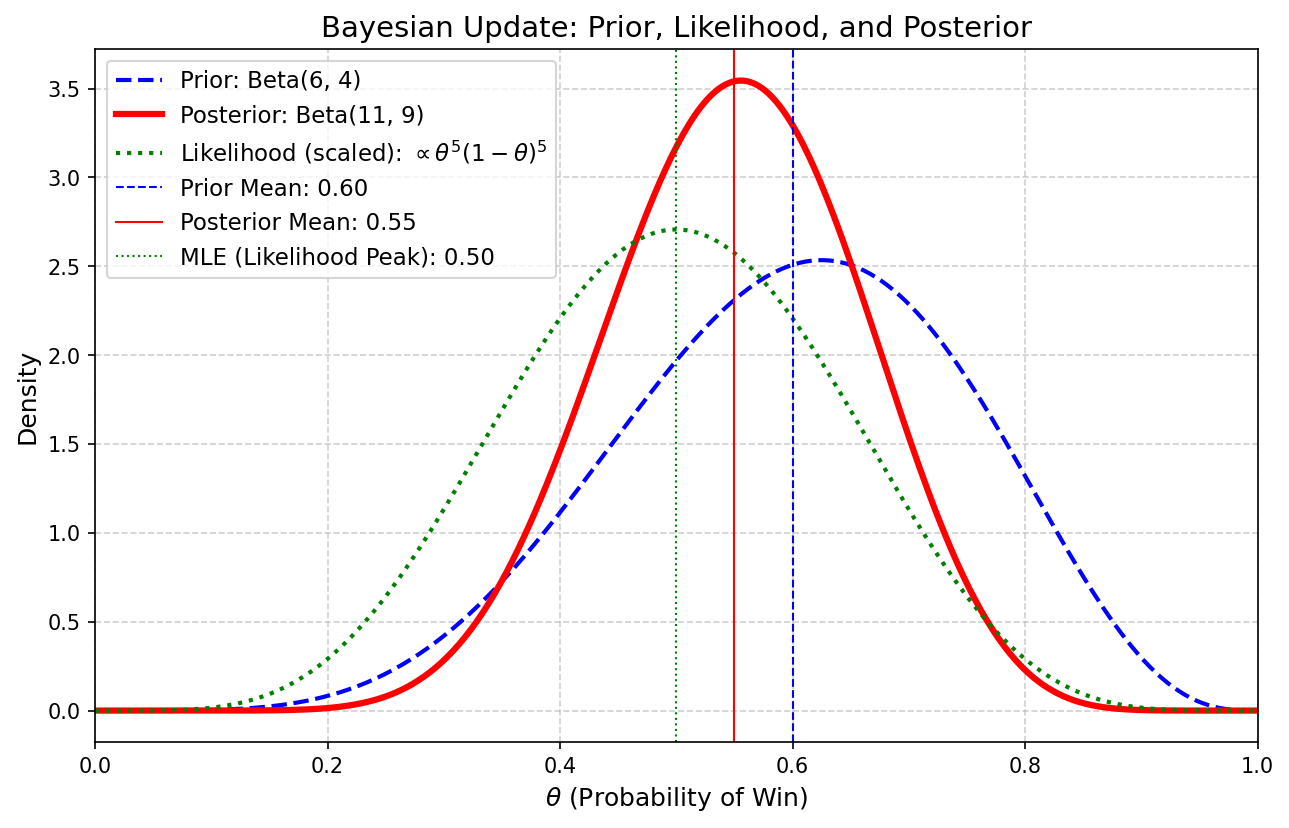
\includegraphics[height=0.75\textheight,width=\textwidth]{q8_d.png}
  \caption{density plot posterior distribution}
\end{figure}
\end{comment}


\noindent\rule{\textwidth}{0.4pt}\\

\newpage


%------------------
% Solution for 9 (a)
%------------------
\subsubsection*{Solution 9}
\noindent\rule{\textwidth}{0.4pt}\\
\subsubsection*{Question 9 (a)}
\begin{flushleft}
\textbf{Accidents per day.} The number of car accidents per day in a big city follows a Poisson($\theta$) distribution. Suppose that we decide to do a Bayesian analysis in which we treat $\theta$ as a random variable whose prior distribution is $\operatorname{Gamma}(1,1)$.\\
Under this prior what is the expected value of $\theta$
\end{flushleft}

\subsubsection*{Solution 9 (a)}

\subsubsection*{\normalfont}{$\therefore$ } \\

\noindent\rule{\textwidth}{0.4pt}\\

\newpage

%------------------
% Solution for 9 (b)
%------------------
\subsubsection*{Solution 9}
\noindent\rule{\textwidth}{0.4pt}\\
\subsubsection*{Question 9 (b)}
\begin{flushleft}
\textbf{Accidents per day.} The number of car accidents per day in a big city follows a Poisson($\theta$) distribution. Suppose that we decide to do a Bayesian analysis in which we treat $\theta$ as a random variable whose prior distribution is $\operatorname{Gamma}(1,1)$.\\
Now we get some data. We count the number of car accidents for ten days, and get the following values:
\end{flushleft}

$$13, 2, 4, 20, 10, 9, 4, 5, 12, 15$$
\begin{flushleft}
Based on these observations, what is the posterior distribution of $\theta$?
\end{flushleft}

\subsubsection*{Solution 9 (b)}

\subsubsection*{\normalfont}{$\therefore$ } \\

\noindent\rule{\textwidth}{0.4pt}\\

\newpage

%------------------
% Solution for 9 (c)
%------------------
\subsubsection*{Solution 9}
\noindent\rule{\textwidth}{0.4pt}\\
\subsubsection*{Question 9 (c)}
\begin{flushleft}
\textbf{Accidents per day.} The number of car accidents per day in a big city follows a Poisson($\theta$) distribution. Suppose that we decide to do a Bayesian analysis in which we treat $\theta$ as a random variable whose prior distribution is $\operatorname{Gamma}(1,1)$.\\
Now we get some data. We count the number of car accidents for ten days, and get the following values:
\end{flushleft}

$$13, 2, 4, 20, 10, 9, 4, 5, 12, 15$$
\begin{flushleft}
Continuing from part (b), plot both the prior and posterior densities.
\end{flushleft}

\subsubsection*{Solution 9 (c)}

\subsubsection*{density plot prior distribution}

\begin{comment}
\begin{figure}[h]
  \includegraphics[height=0.75\textheight,width=\textwidth]{q9_c_prior.png}
  \caption{density plot prior distribution}
\end{figure}
\end{comment}

\subsubsection*{density plot posterior distribution}

\begin{comment}
\begin{figure}[h]
  \includegraphics[height=0.75\textheight,width=\textwidth]{q9_c_posterior.png}
  \caption{density plot posterior distribution}
\end{figure}
\end{comment}

\subsubsection*{\normalfont}{$\therefore$ } \\

\noindent\rule{\textwidth}{0.4pt}\\

\newpage

%------------------
% Solution for 10 (a)
%------------------
\subsubsection*{Solution 10}
\noindent\rule{\textwidth}{0.4pt}\\
\subsubsection*{Question 10 (a)}
\begin{flushleft}
In an election, there are three candidates, $A, B$, and $C$. Of the voting population, $\theta_{A}$ fraction will vote for $A$, while $\theta_{B}$ fraction will vote for $B$ and $\theta_{C}$ fraction will vote for $C$; thus $\theta_{A}+\theta_{B}+\theta_{C}=1$.\\

John wishes to infer the distribution $\left(\theta_{A}, \theta_{B}, \theta_{C}\right)$. He starts by putting a uniform prior on it; that is, he considers all distributions to be equally likely. He then picks four people at random to poll, and finds that they intend to vote for $A, B, B, A$, respectively. Given this information, what is John's posterior distribution?
\end{flushleft}

\subsubsection*{Solution 10 (a)}

\subsubsection*{\normalfont}{$\therefore$ } \\

\noindent\rule{\textwidth}{0.4pt}\\

\newpage

%------------------
% Solution for 10 (b)
%------------------
\subsubsection*{Solution 10}
\noindent\rule{\textwidth}{0.4pt}\\
\subsubsection*{Question 10 (b)}
\begin{flushleft}
In an election, there are three candidates, $A, B$, and $C$. Of the voting population, $\theta_{A}$ fraction will vote for $A$, while $\theta_{B}$ fraction will vote for $B$ and $\theta_{C}$ fraction will vote for $C$; thus $\theta_{A}+\theta_{B}+\theta_{C}=1$.\\

Under this posterior distribution, what is the expected value of $\left(\theta_{A}, \theta_{B}, \theta_{C}\right)$?
\end{flushleft}


\subsubsection*{Solution 10 (b)}

\subsubsection*{\normalfont}{$\therefore$ } \\

\noindent\rule{\textwidth}{0.4pt}\\

\newpage

\end{document}

\begin{comment}
%------------------
% Solution for 2(a),2(b), and 2(c)
%------------------
\subsection*{Solution 2}
\noindent\rule{\textwidth}{0.4pt}\\
\subsubsection*{Solution 2 (a)}
\subsubsection*{Step 1: Define Euclidean distance ($\ell_2$)}
\parbox{\textwidth}{

$$\ell_2 = \|p - q\|_2 = \sqrt{\sum_{i=1}^{n} (p_i - q_i)^2}$$

}

\subsubsection*{Step 2: Compute $\ell_2$}
\parbox{\textwidth}{
Let $p=1$ and $q=10$
$$
\begin{aligned}
\ell_2 &= \sqrt{\sum_{i=1}^{n} (p_i - q_i)^2}\\
\ell_2 &= \sqrt{\sum_{i=1}^{1} (1 - 10)^2}\\
\ell_2 &= \sqrt{(- 9)^2}\\
\ell_2 &= 9
\end{aligned}
$$
}
\subsubsection*{\normalfont}{$\therefore$ $\ell_{2} = 9$}

\noindent\rule{\textwidth}{0.4pt}\\

\subsubsection*{Solution 2 (b)}
\subsubsection*{Step 1: Define Euclidean distance ($\ell_2$)}
\parbox{\textwidth}{

$$\ell_2 = \|p - q\|_2 = \sqrt{\sum_{i=1}^{n} (p_i - q_i)^2}$$

}

\subsubsection*{Step 2: Compute $\ell_2$}
\parbox{\textwidth}{
Let $p = \begin{bmatrix} -1 \\ 12 \end{bmatrix}, q = \begin{bmatrix} 6 \\ -12 \end{bmatrix}$
$$
\begin{aligned}
\ell_2 &= \sqrt{\sum_{i=1}^{n} (p_i - q_i)^2}\\
\ell_2 &= \sqrt{(p_1 - q_1)^{2}+(p_2 - q_2)^{2}}\\
\ell_2 &= \sqrt{(-1 - 6)^{2}+(12 - (-12))^{2}}\\
\ell_2 &= \sqrt{(-7)^{2}+(24)^{2}}\\
\ell_2 &= \sqrt{625}\\
\ell_2 &= 25
\end{aligned}
$$
}
\subsubsection*{\normalfont}{$\therefore$ $\ell_{2} = 25$}

\noindent\rule{\textwidth}{0.4pt}\\


\subsection*{Solution 2}
\noindent\rule{\textwidth}{0.4pt}\\
\subsubsection*{Solution 2 (c)}
\subsubsection*{Step 1: Define Euclidean distance ($\ell_2$)}
\parbox{\textwidth}{

$$\ell_2 = \|p - q\|_2 = \sqrt{\sum_{i=1}^{n} (p_i - q_i)^2}$$

}

\subsubsection*{Step 2: Compute $\ell_2$}
\parbox{\textwidth}{
Let $p = \begin{bmatrix} 1 \\ 5 \\ -1 \end{bmatrix}, q = \begin{bmatrix} 5 \\ 2 \\ 11 \end{bmatrix}$
$$
\begin{aligned}
\ell_2 &= \sqrt{\sum_{i=1}^{n} (p_i - q_i)^2}\\
\ell_2 &= \sqrt{(p_1 - q_1)^{2}+(p_2 - q_2)^{2}+(p_3 - q_3)^{2}}\\
\ell_2 &= \sqrt{(1 - 5)^{2}+(5 - 2)^{2}+(-1 - 11)^{2}}\\
\ell_2 &= \sqrt{(-4)^{2}+(3)^{2}+(-12)^{2}}\\
\ell_2 &= \sqrt{169}\\
\ell_2 &= 13
\end{aligned}
$$
}
\subsubsection*{\normalfont}{$\therefore$ $\ell_{2} = 13$}

\noindent\rule{\textwidth}{0.4pt}\\

\newpage

%------------------
% Solution for 3(a) and 3(b)
%------------------
\subsection*{Solution 3}
\noindent\rule{\textwidth}{0.4pt}\\
\subsubsection*{Solution 3 (a)}
\subsubsection*{Step 1: Normalize the vector $x$}
\parbox{\textwidth}{
Let $x = \begin{bmatrix} 10 \\ 15 \\ 25 \end{bmatrix}$

$$\sum_{i=1}^{3} x_{i} = x_{1} + x_{2} + x_{3} = 10 + 15 + 25 = 50$$

Now, divide each entry by the total sum:\\

$$p = \frac{1}{50} \cdot x = \frac{1}{50} \begin{bmatrix} 10 \\ 15 \\ 25 \end{bmatrix} = \begin{bmatrix} 10/50 \\ 15/50 \\ 25/50 \end{bmatrix} = \begin{bmatrix} 0.2 \\ 0.3 \\ 0.5 \end{bmatrix}$$
}
\subsubsection*{\normalfont}{$\therefore$ the result ($p$) of scaling vertor $x$ is the following:}
$$p = \begin{bmatrix} 0.2 \\ 0.3 \\ 0.5 \end{bmatrix}$$ \\

\noindent\rule{\textwidth}{0.4pt}\\

\subsubsection*{Solution 3 (b)}
\subsubsection*{Step 1: Define dimension of the probability simplex}
\parbox{\textwidth}{
The dimension of vector $p$ is $3$ and $k=n-1$ where $k$ is the dimension of the probability simplex
}
\subsubsection*{\normalfont}{$\therefore$ vector $p$ lies in the probability simplex($\Delta_2$) for $k=2$}

\noindent\rule{\textwidth}{0.4pt}\\

\newpage

%------------------
% Solution for 4
%------------------
\subsection*{Solution 4}
\noindent\rule{\textwidth}{0.4pt}\\

\subsubsection*{Step 1: Define probability simplex $\Delta_2$ }
\parbox{\textwidth}{

For a point to be scalable to $\Delta_2$, after scaling it must satisfy:
\begin{itemize}
\item All components must be non-negative
\item The sum of components must equal 1
\end{itemize}
}

\subsubsection*{Step 2: Give example that violates one of the rules in Step 1}
\parbox{\textwidth}{
Let $x = \begin{bmatrix} 1 \\ -2 \end{bmatrix}$

The second component of $x$ violates the first rule, all components for a point must be non-negative $\Delta_2$.
}

\subsubsection*{\normalfont}{$\therefore$ the point $x = \begin{bmatrix} 1 \\ -2 \end{bmatrix}$ cannot be scaled to lie in $\Delta_{2}$}

\noindent\rule{\textwidth}{0.4pt}\\

\newpage

%------------------
% Solution for 5
%------------------
\subsection*{Solution 5}
\noindent\rule{\textwidth}{0.4pt}\\

\subsubsection*{Visualizing the Simplex $\Delta_3$ in 2D Projections}
\parbox{\textwidth}{
Here are the three 2D views of the probability simplex $\Delta_3$. Each plot is a \textit{shadow} of the 3D triangle, viewed along one of the principal axes.
}

%---------------------------------------------------
%  FIGURE 1: x1 vs x2 Projection
%---------------------------------------------------
\begin{figure}[h!]
\centering
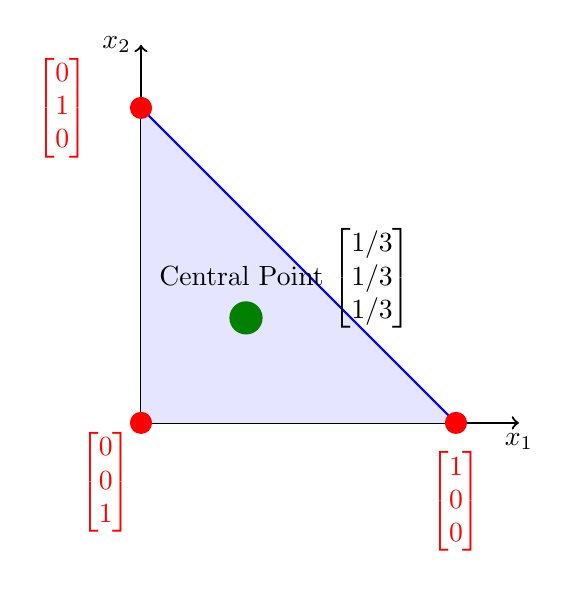
\begin{tikzpicture}[scale=4]
    % Axes
    \draw[->, thick] (0,0) -- (1.2,0) node[below] {$x_1$};
    \draw[->, thick] (0,0) -- (0,1.2) node[left] {$x_2$};

    % The projected simplex region (x1 + x2 <= 1)
    \fill[blue!10] (0,0) -- (1,0) -- (0,1) -- cycle;
    \draw[blue, thick] (1,0) -- (0,1);

    % The three vertices of the simplex
    \fill[red] (1,0) circle (1pt) node[shift={(0, -1)}] {$\begin{bmatrix} 1 \\ 0 \\ 0 \end{bmatrix}$};
    \fill[red] (0,1) circle (1pt) node[shift={(-1, 0)}] {$\begin{bmatrix} 0 \\ 1 \\ 0 \end{bmatrix}$};
    \fill[red] (0,0) circle (1pt) node[below left] {$\begin{bmatrix} 0 \\ 0 \\ 1 \end{bmatrix}$};

    % The central point (centroid)
    \fill[green!50!black] (1/3, 1/3) circle (1.5pt) node[shift={(0.5,0.5)}, black] {Central Point $\begin{bmatrix} 1/3 \\ 1/3 \\ 1/3 \end{bmatrix}$};
\end{tikzpicture}
\caption{View 1: Projection onto the $x_1$-$x_2$ plane.}
\label{fig:x1x2}
\end{figure}

%---------------------------------------------------
%  FIGURE 2: x2 vs x3 Projection
%---------------------------------------------------
\begin{figure}[h!]
\centering
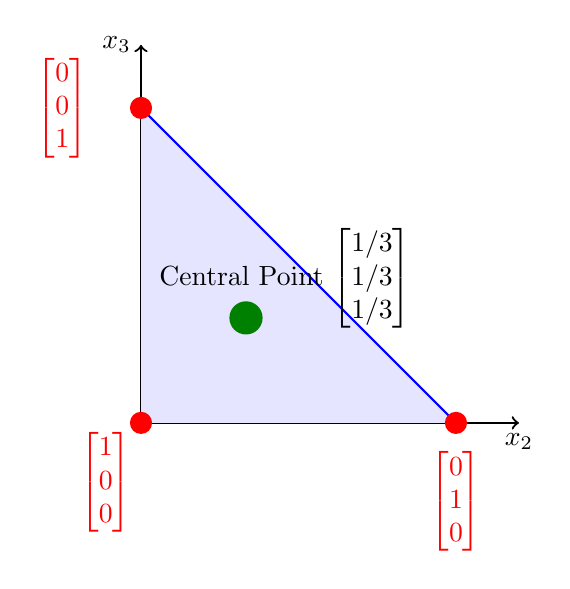
\begin{tikzpicture}[scale=4]
    % Axes
    \draw[->, thick] (0,0) -- (1.2,0) node[below] {$x_2$};
    \draw[->, thick] (0,0) -- (0,1.2) node[left] {$x_3$};

    % The projected simplex region (x2 + x3 <= 1)
    \fill[blue!10] (0,0) -- (1,0) -- (0,1) -- cycle;
    \draw[blue, thick] (1,0) -- (0,1);

    % The three vertices of the simplex
    \fill[red] (1,0) circle (1pt) node[shift={(0, -1)}] {$\begin{bmatrix} 0 \\ 1 \\ 0 \end{bmatrix}$};
    \fill[red] (0,1) circle (1pt) node[shift={(-1, 0)}] {$\begin{bmatrix} 0 \\ 0 \\ 1 \end{bmatrix}$};
    \fill[red] (0,0) circle (1pt) node[below left] {$\begin{bmatrix} 1 \\ 0 \\ 0 \end{bmatrix}$};

    % The central point (centroid)
    \fill[green!50!black] (1/3, 1/3) circle (1.5pt) node[shift={(0.5,0.5)}, black] {Central Point $\begin{bmatrix} 1/3 \\ 1/3 \\ 1/3 \end{bmatrix}$};
\end{tikzpicture}
\caption{View 2: Projection onto the $x_2$-$x_3$ plane.}
\label{fig:x2x3}
\end{figure}

\newpage

\subsection*{Solution 5}
\noindent\rule{\textwidth}{0.4pt}\\
%---------------------------------------------------
%  FIGURE 3: x1 vs x3 Projection
%---------------------------------------------------
\begin{figure}[h!]
\centering
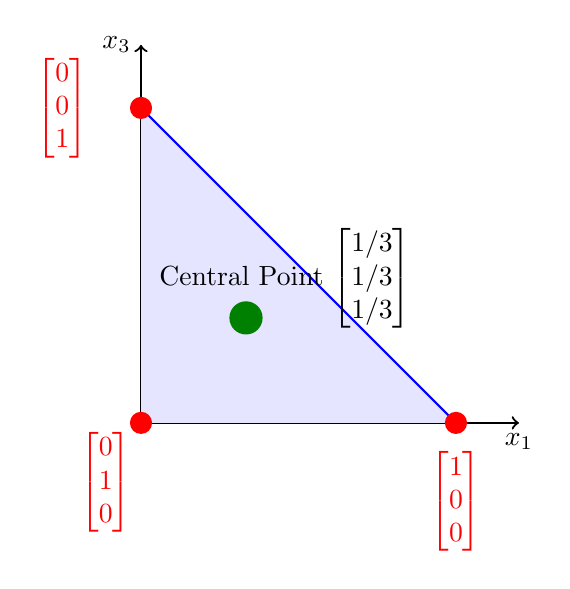
\begin{tikzpicture}[scale=4]
    % Axes
    \draw[->, thick] (0,0) -- (1.2,0) node[below] {$x_1$};
    \draw[->, thick] (0,0) -- (0,1.2) node[left] {$x_3$};

    % The projected simplex region (x1 + x3 <= 1)
    \fill[blue!10] (0,0) -- (1,0) -- (0,1) -- cycle;
    \draw[blue, thick] (1,0) -- (0,1);

    % The three vertices of the simplex
    \fill[red] (1,0) circle (1pt) node[shift={(0, -1)}] {$\begin{bmatrix} 1 \\ 0 \\ 0 \end{bmatrix}$};
    \fill[red] (0,1) circle (1pt) node[shift={(-1, 0)}] {$\begin{bmatrix} 0 \\ 0 \\ 1 \end{bmatrix}$};
    \fill[red] (0,0) circle (1pt) node[below left] {$\begin{bmatrix} 0 \\ 1 \\ 0 \end{bmatrix}$};

    % The central point (centroid)
    \fill[green!50!black] (1/3, 1/3) circle (1.5pt) node[shift={(0.5,0.5)}, black] {Central Point $\begin{bmatrix} 1/3 \\ 1/3 \\ 1/3 \end{bmatrix}$};
\end{tikzpicture}
\caption{View 3: Projection onto the $x_1$-$x_3$ plane.}
\label{fig:x1x3}
\end{figure}

\noindent\rule{\textwidth}{0.4pt}\\

\newpage

%------------------
% Solution for 6
%------------------
\subsection*{Solution 6}
\noindent\rule{\textwidth}{0.4pt}\\

\subsubsection*{6 (a): $\ell_1$ for $p$ and $q$}

\parbox{\textwidth}{The $\ell_1$ distance between two vectors $p, q \in \mathbb{R}^n$ is given by:
$$\|p-q\|_1 = \sum_{i=1}^n |p_i - q_i|$$

Let $p = \begin{bmatrix} 1/2 \\ 1/4 \\ 1/8 \\ 1/8 \end{bmatrix}$ and $q = \begin{bmatrix} 1/4 \\ 1/4 \\ 1/4 \\ 1/4 \end{bmatrix}$

\begin{align*}
    \|p-q\|_1 &= \left|\frac{1}{2} - \frac{1}{4}\right| + \left|\frac{1}{4} - \frac{1}{4}\right| + \left|\frac{1}{8} - \frac{1}{4}\right| + \left|\frac{1}{8} - \frac{1}{4}\right| \\
    &= \left|\frac{2}{4} - \frac{1}{4}\right| + |0| + \left|\frac{1}{8} - \frac{2}{8}\right| + \left|\frac{1}{8} - \frac{2}{8}\right| \\
    &= \frac{1}{4} + 0 + \left|-\frac{1}{8}\right| + \left|-\frac{1}{8}\right| \\
    &= \frac{1}{4} + \frac{1}{8} + \frac{1}{8} = \frac{2}{8} + \frac{1}{8} + \frac{1}{8} = \frac{4}{8} = \frac{1}{2}
\end{align*}
}
\subsubsection*{\normalfont}{$\therefore$ $\ell_{1}= \frac{1}{2}$}

\noindent\rule{\textwidth}{0.4pt}\\

\newpage

\subsection*{Solution 6}
\noindent\rule{\textwidth}{0.4pt}\\

\subsubsection*{6 (b): $\ell_1$ for $q$ and $r$}
\parbox{\textwidth}{The $\ell_1$ distance between two vectors $q, r \in \mathbb{R}^n$ is given by:
$$\|q-r\|_1 = \sum_{i=1}^n |q_i - r_i|$$

Let $q = \begin{bmatrix} 1/4 \\ 1/4 \\ 1/4 \\ 1/4 \end{bmatrix}$ and $r = \begin{bmatrix} 1/2 \\ 0 \\ 1/4 \\ 1/4 \end{bmatrix}$

\begin{align*}
\|q-r\|_1 &= \sum_{i=1}^{4} |q_i - r_i| \\
&= \left|\frac{1}{4} - \frac{1}{2}\right| + \left|\frac{1}{4} - 0\right| + \left|\frac{1}{4} - \frac{1}{4}\right| + \left|\frac{1}{4} - \frac{1}{4}\right| \\
&= \left|\frac{1}{4} - \frac{2}{4}\right| + \left|\frac{1}{4}\right| + |0| + |0| \\
&= \left|-\frac{1}{4}\right| + \frac{1}{4} + 0 + 0 \\
&= \frac{1}{4} + \frac{1}{4} \\
&= \frac{1}{2}
\end{align*}
}

\subsubsection*{\normalfont}{$\therefore$ $\ell_1 = \frac{1}{2}$}

\noindent\rule{\textwidth}{0.4pt}\\

\newpage

\subsection*{Solution 6}
\noindent\rule{\textwidth}{0.4pt}\\

\subsubsection*{6 (c): KL divergence $K(p, q)$}
\parbox{\textwidth}{
The Kullback-Leibler (KL) divergence from a distribution $p$ to a distribution $q$ is defined as:
$$K(p, q) = \sum_{i} p_i \ln \frac{p_i}{q_i}$$
Let $p = \begin{bmatrix} 1/2 \\ 1/4 \\ 1/8 \\ 1/8 \end{bmatrix}$ and $q = \begin{bmatrix} 1/4 \\ 1/4 \\ 1/4 \\ 1/4 \end{bmatrix}$
}

\begin{align*}
K(p, q) &= \sum_{i=1}^{4} p_i \ln\left(\frac{p_i}{q_i}\right) \\
&= p_1 \ln\left(\frac{p_1}{q_1}\right) + p_2 \ln\left(\frac{p_2}{q_2}\right) + p_3 \ln\left(\frac{p_3}{q_3}\right) + p_4 \ln\left(\frac{p_4}{q_4}\right) \\
&= \frac{1}{2}\ln\left(\frac{1/2}{1/4}\right) + \frac{1}{4}\ln\left(\frac{1/4}{1/4}\right) + \frac{1}{8}\ln\left(\frac{1/8}{1/4}\right) + \frac{1}{8}\ln\left(\frac{1/8}{1/4}\right) \\
&= \frac{1}{2}\ln(2) + \frac{1}{4}\ln(1) + \frac{1}{8}\ln\left(\frac{1}{2}\right) + \frac{1}{8}\ln\left(\frac{1}{2}\right) \\
&= \frac{1}{2}\ln(2) + \frac{1}{4}(0) - \frac{1}{8}\ln(2) - \frac{1}{8}\ln(2) \\
&= \frac{1}{2}\ln(2) - \frac{2}{8}\ln(2) \\
&= \left(\frac{1}{2} - \frac{1}{4}\right)\ln(2) \\
&= \frac{1}{4}\ln(2)
\end{align*}

\subsubsection*{\normalfont{$\therefore$ $K(p,q) = \frac{1}{4}\ln(2)$}}
\noindent\rule{\textwidth}{0.4pt}\\

\newpage

\subsection*{Solution 6}
\noindent\rule{\textwidth}{0.4pt}\\

\subsubsection*{6 (d): KL divergence $K(q, r)$}
\parbox{\textwidth}{
The Kullback-Leibler (KL) divergence from a distribution $q$ to a distribution $r$ is defined as:
$$K(q, r) = \sum_{i} q_i \ln \frac{q_i}{r_i}$$
Let $q = \begin{bmatrix} 1/4 \\ 1/4 \\ 1/4 \\ 1/4 \end{bmatrix}$ and $r = \begin{bmatrix} 1/2 \\ 0 \\ 1/4 \\ 1/4 \end{bmatrix}$ \\

Looking at the second component ($i=2$). Here, $q_2 = \frac{1}{4} > 0$ while $r_2 = 0$. The corresponding term in the KL divergence sum, $q_2 \ln\left(\frac{q_2}{r_2}\right)$, involves division by zero. \\

Hence, the divergence will be infinite.
}
\subsubsection*{\normalfont}{$\therefore$ $K(q, r) = \infty$}

\noindent\rule{\textwidth}{0.4pt}\\

\newpage
%------------------
% Solution for 7
%------------------
\subsection*{Solution 7}
\noindent\rule{\textwidth}{0.4pt}\\

\subsubsection*{Python Code}
\begin{lstlisting}
import numpy as np
import matplotlib.pyplot as plt
from extract_feature import compute_or_load_features
from sklearn.neighbors import KNeighborsClassifier

def run_nearest_neighbor(x_train, y_train, x_test, y_test):
    # create classifier    
    nn_classifier = KNeighborsClassifier(n_neighbors=1, algorithm='auto')

    # train 
    nn_classifier.fit(x_train, y_train)

    # test and report accuracy
    test_acc = nn_classifier.score(x_test, y_test)

    print("Nearest neighbor accuracy on the test set: %f"%test_acc)

    return nn_classifier


def analyze_nn(classifier, x_train, y_train, x_test, y_test, x_test_features, N, model_type):
    """
    generalization to grab indices, predictions, and make plots
    """
    # list of image labels
    CIFAR_CLASSES = ['airplane', 'automobile', 'bird', 'cat', 'deer', 'dog', 'frog', 'horse', 'ship', 'truck']

    # get predictions of classifier on test data
    y_pred = classifier.predict(x_test_features)
    
    # define bool condtion where classifier made correct prediction
    is_correct = (y_pred == y_test)
    
    # get indices for correct and incorrect samples
    correct_indices_test = np.where(is_correct)[0][:N]
    incorrect_indices_test = np.where(~is_correct)[0][:N]
    
    # make image plots 
    def plot_pairs(title, test_indices):
        
        # check just in case of bad result.. nema nista
        if len(test_indices) == 0:
            return
            
        # Get the feature vectors for the selected test images (flattened)
        selected_test_features = x_test_features[test_indices]
        
        # get nearest neighbor
        # note: kneighbors -> (distances, indices).. only need the indices.
        _, nn_train_indices_2D = classifier.kneighbors(X=selected_test_features, n_neighbors=1)
        
        # 2D -> 1D
        nn_train_indices = nn_train_indices_2D.flatten()
        
        # get images and labels for the selected test points
        test_images_sample = x_test[test_indices]
        test_labels_sample = y_test[test_indices]
        
        #get the RAW neighbor image and label from the training points
        nn_images_sample = x_train[nn_train_indices]
        nn_labels_sample = y_train[nn_train_indices]
        
        # prediction is nearest neighbor label
        y_pred_sample = nn_labels_sample
        
        # reshape (N, C, H, W) to (N, H, W, C) for plot
        test_images_plt = test_images_sample.transpose(0, 2, 3, 1)
        nn_images_plt = nn_images_sample.transpose(0, 2, 3, 1)

        N_plot = len(test_indices)
        
        # just in case only 1 image is plotted (axes will be 1D instead of 2D)
        if N_plot == 1:
            fig, axes = plt.subplots(N_plot, 2, figsize=(6, 2))
            axes = axes[np.newaxis, :] 
        else:
            fig, axes = plt.subplots(N_plot, 2, figsize=(6, 2 * N_plot))
            
        fig.suptitle(title, fontsize=14, y=1.02)
        
        for i in range(N_plot):
            is_correct = (test_labels_sample[i] == y_pred_sample[i])
            pred_color = 'green' if is_correct else 'red'
            
            # plot test image
            axes[i, 0].imshow(test_images_plt[i] / 255.0)
            axes[i, 0].set_title(f"Test ({CIFAR_CLASSES[test_labels_sample[i]]})", fontsize=10)
            axes[i, 0].axis('off')
            
            # plot nearest neighbor
            axes[i, 1].imshow(nn_images_plt[i] / 255.0)
            axes[i, 1].set_title(
                f"NN ({CIFAR_CLASSES[nn_labels_sample[i]]})", 
                fontsize=10, 
                color=pred_color
            )
            axes[i, 1].axis('off')
        
        plt.tight_layout(rect=[0, 0.03, 1, 0.98])
        plt.show()
        fig.savefig(f"{title.split(' ')[2].lower()}_{model_type}.png")

    # plot correct and incorrect cases
    plot_pairs(f"First {N} Correct Predictions ({model_type})", correct_indices_test)
    plot_pairs(f"First {N} Incorrect Predictions ({model_type})", incorrect_indices_test)

# raw pixel 
raw_pixel_train_features, raw_pixel_test_features = compute_or_load_features(x_train, x_test, "raw_pixel")
raw_pixel_knn_classifier = run_nearest_neighbor(raw_pixel_train_features, y_train, raw_pixel_test_features, y_test)
analyze_nn(
    classifier=raw_pixel_knn_classifier,
    x_train=x_train,  
    y_train=y_train,
    x_test=x_test,    
    y_test=y_test,
    x_test_features=raw_pixel_test_features, 
    N=5,
    model_type="raw_pixel"
)

# HoG
hog_train_features, hog_test_features = compute_or_load_features(x_train, x_test, "hog")
hog_knn_classifier = run_nearest_neighbor(hog_train_features, y_train, hog_test_features, y_test)
analyze_nn(
    classifier=hog_knn_classifier,
    x_train=x_train,  
    y_train=y_train,
    x_test=x_test,    
    y_test=y_test,
    x_test_features=hog_test_features, 
    N=5,
    model_type="hog"
)

# vgg-last-fc
pretrained_cnn_last_fc_train_features, pretrained_cnn_last_fc_test_features = compute_or_load_features(x_train, x_test, "pretrained_cnn", "last_fc")
pretrained_cnn_last_fc_knn_classifier = run_nearest_neighbor(pretrained_cnn_last_fc_train_features, y_train, pretrained_cnn_last_fc_test_features, y_test)
analyze_nearest_neighbors_simple(
    classifier=pretrained_cnn_last_fc_knn_classifier,
    x_train=x_train,  
    y_train=y_train,
    x_test=x_test,    
    y_test=y_test,
    x_test_features=pretrained_cnn_last_fc_test_features, 
    N=5,
    model_type='vgg_last_fc'
)
\end{lstlisting}

\newpage
\subsection*{Solution 7}
\subsubsection*{Part a: Dimensionality for each of the representations (raw pixel, HoG, VGG-last-fc, VGG-last-conv)}
\begin{center} 
  \begin{tabular}{|c|c|} 
    \hline Feature Type & Dimensionality \\ 
    \hline 
    Raw Pixel & 3072 \\ 
    HoG & 512  \\
    VGG-last-fc & 4096 \\
    VGG-last-conv & 512 \\ 
    \hline
  \end{tabular}
\end{center}

\noindent\rule{\textwidth}{0.4pt}\\

\subsubsection*{Part b: Test accuracies for 1-nearest neighbor classification using the various representations (raw pixel, HoG, VGG-last-fc, VGG-last-conv, random-VGG-last-fc, random-VGG-last-conv).}
\begin{center} 
  \begin{tabular}{|c|c|} 
    \hline Feature Type & 1-NN test accuracy (\%) \\ 
    \hline 
    Raw Pixel & 35.4 \\ 
    HoG & 36.6  \\
    VGG-last-fc & 92.1 \\
    VGG-last-conv & 92.0 \\
    random VGG-last-fc & 39.1 \\
    random VGG-last-conv & 40.6 \\ 
    \hline
  \end{tabular}
\end{center}
\noindent\rule{\textwidth}{0.4pt}\\

\newpage

\subsection*{Solution 7}
\noindent\rule{\textwidth}{0.4pt}\\
\subsubsection*{Part c:  Raw Pixel correct/incorrect}

\begin{figure}[h]
  
\includegraphics[height=0.75\textheight,width=\textwidth]{raw_pixel.png}
  \caption{First five correct/incorrect images for Raw Pixel}
\end{figure}

\newpage

\subsection*{Solution 7}
\noindent\rule{\textwidth}{0.4pt}\\
\subsubsection*{Part c:  HoG correct/incorrect}

\begin{figure}[h]
  
\includegraphics[height=0.75\textheight,width=\textwidth]{hog.png}
  \caption{First five correct/incorrect images for HoG}
\end{figure}

\newpage

\subsection*{Solution 7}
\noindent\rule{\textwidth}{0.4pt}\\
\subsubsection*{Part c:  VGG-last-fc correct/incorrect}

\begin{figure}[h]
  
\includegraphics[height=0.75\textheight,width=\textwidth]{vgg_last_fc.png}
  \caption{First five correct/incorrect images for VGG-last-fc}
\end{figure}

\newpage

\subsection*{Solution 8}
\noindent\rule{\textwidth}{0.4pt}\\

\subsubsection*{Python Code}
\begin{lstlisting}
import numpy as np
from sklearn.neighbors import NearestNeighbors

filename = 'glove.6B.300d.txt'
with open(filename) as f:
    content = f.read().splitlines()

# initialize vecs and words 'containers'
n = len(content)
vecs = np.zeros((n, 300))
words = ["" for i in range(n)] 
for index, rawline in enumerate(content):
    line = rawline.split()
    words[index] = line[0]
    # need4numpy speed
    vecs[index] = np.array(line[1:], dtype=np.float32)

# make dict for access to word and index
word_to_index = {word: i for i, word in enumerate(words)}

# initialize target words
target_words = ['communism', 'africa', 'happy', 'sad', 'upset', 'computer', 'cat', 'dollar']

# find 5 nearest neighbors (n).. remember k = n+1
n_neighbors = 6

# initialize  and fit the nn model
nn_model = NearestNeighbors(n_neighbors=n_neighbors, metric='euclidean', algorithm='auto')
nn_model.fit(vecs)

# gracefully check for typo
try:
    target_indices = [word_to_index[word] for word in target_words]
except KeyError as e:
    print(f" error: word '{e.args[0]}' was not found.")
    exit()

# extract the corresponding vectors for the target words from vecs
target_vectors = vecs[target_indices]

# find the nearest neighbors
distances, indices = nn_model.kneighbors(target_vectors)

# format and print results
results = {}
for i, word in enumerate(target_words):
    neighbor_indices = indices[i][1:]
    neighbor_words = [words[idx] for idx in neighbor_indices]
    results[word] = neighbor_words

print(f"5 nearest neighbors in {filename} for {target_words}")
print(results)

\end{lstlisting}

\newpage 
\subsection*{Solution 8}
\noindent\rule{\textwidth}{0.4pt}\\
\subsubsection*{Word Vectors: 5 closest words}
\begin{center} 
  \begin{tabular}{|c|c|} 
    \hline Target Word & Five Closest Words \\ 
    \hline 
    communism & \text{['fascism', 'capitalism', 'nazism', 'stalinism', 'socialism']} \\ 
    africa & \text{['african', 'continent', 'south', 'africans', 'zimbabwe']}  \\
    happy & \text{['glad', 'pleased', 'always', 'everyone', 'sure']} \\
    sad & \text{['sorry', 'tragic', 'happy', 'pathetic', 'awful']} \\ 
    upset & \text{['upsetting', 'surprised', 'upsets', 'stunned', 'shocked']}\\
    computer & \text{['computers', 'software', 'technology', 'laptop', 'computing']}\\
    cat & \text{['cats', 'dog', 'pet', 'feline', 'dogs']}\\
    dollar & \text{['currency', 'dollars', 'euro', 'multibillion', 'weaker']}\\

    \hline
  \end{tabular}
\end{center}

\noindent\rule{\textwidth}{0.4pt}\\

\end{comment}


\end{document}